% !TEX TS-program = pdflatex
% !TEX encoding = UTF-8 Unicode
% 
% This is a simple template for a LaTeX document using the "article" class.
% See "book", "report", "letter" for other types of document.
% 
\documentclass[11pt]{article} % use larger type; default would be 10pt
% 
% 
% 
%%% The "real" document content comes below...
\input{header}
% 
\title{Introduction to Math for DS Group Task 1}
\author{IMDS Group 24 \\ Zehao Qian, Mohammad Jamshaid Iqbal, Chloe Mendez}
\begin{document}
\maketitle
% 
% 
% \input{example}
\section{Question 1}
\paragraph{Consider the line L in $R^3$ passing through the origin and the point P=(2,2,1)? Which of the following points is closest to L, and which is farthest from L?}
\begin{itemize}
    \item A: (8, 9, 0.9)
    \item B: (4, 4, 2.1)
    \item C: (0.9, 0.99, 0.49)
    \item D: (-2, -2, 1)
    \item E: (0, 2.1, 0)
\end{itemize}

\subsection{Analytics:}
\paragraph{In three-dimensional space, we can calculate the distance from a point to a line using the following formula:}
\paragraph{Let's say you have a point P with coordinates $(x_0, y_0, z_0)$, and a line defined by two points A$(x_1, y_1, z_1)$ and B$(x_2, y_2, z_2)$. The formula to calculate the distance (d) from point P to the line AB is as follows:}
% 
% 
$$ d = \frac{|(\mathbf{P} - \mathbf{A}) \cdot \mathbf{n}|}{|\mathbf{AB}|} $$
% 
% 
\paragraph{Here's an explanation of the formula components:}
% 
% 
\begin{itemize}
    \item \(\mathbf{P} - \mathbf{A}\) represents the vector from point A to point P.
    \item \(\mathbf{AB}\) represents the vector along the line from point A to point B.
    \item \(\cdot\) denotes the dot product between vectors.
    \item \(\mathbf{n}\) is the unit vector along the line AB, which is given by \(\frac{\mathbf{AB}}{|\mathbf{AB}|}\).
\end{itemize}
% 
% 
\tikzset{every picture/.style={line width=0.75pt}} %set default line width to 0.75pt        

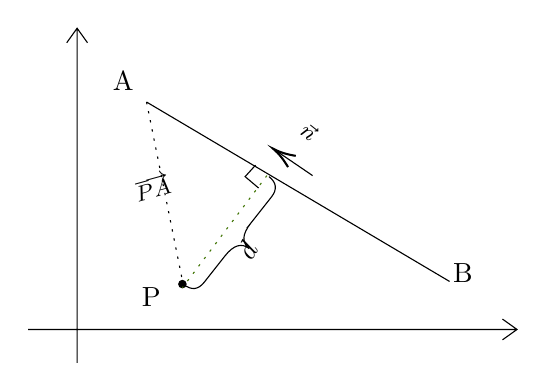
\begin{tikzpicture}[x=0.75pt,y=0.75pt,yscale=-1,xscale=1]
    %uncomment if require: \path (0,210); %set diagram left start at 0, and has height of 210

    %Shape: Axis 2D [id:dp44317292301248945] 
    \draw  (50,159.58) -- (285.5,159.58)(73.55,14.45) -- (73.55,175.7) (278.5,154.58) -- (285.5,159.58) -- (278.5,164.58) (68.55,21.45) -- (73.55,14.45) -- (78.55,21.45)  ;
    %Straight Lines [id:da2979242010824248] 
    \draw    (107,50) -- (253,136.45) ;
    %Shape: Circle [id:dp023999541748674025] 
    \draw  [fill={rgb, 255:red, 0; green, 0; blue, 0 }  ,fill opacity=1 ] (122.5,137.73) .. controls (122.5,136.75) and (123.29,135.95) .. (124.27,135.95) .. controls (125.25,135.95) and (126.05,136.75) .. (126.05,137.73) .. controls (126.05,138.71) and (125.25,139.5) .. (124.27,139.5) .. controls (123.29,139.5) and (122.5,138.71) .. (122.5,137.73) -- cycle ;
    %Straight Lines [id:da4396600304527325] 
    \draw    (187,85.45) -- (169.65,73.63) ;
    \draw [shift={(168,72.5)}, rotate = 34.28] [color={rgb, 255:red, 0; green, 0; blue, 0 }  ][line width=0.75]    (10.93,-3.29) .. controls (6.95,-1.4) and (3.31,-0.3) .. (0,0) .. controls (3.31,0.3) and (6.95,1.4) .. (10.93,3.29)   ;
    %Straight Lines [id:da11083812462923981] 
    \draw  [dash pattern={on 0.84pt off 2.51pt}]  (107,50) -- (124.27,135.95) ;
    %Straight Lines [id:da3033500048537672] 
    \draw [color={rgb, 255:red, 65; green, 117; blue, 5 }  ,draw opacity=1 ] [dash pattern={on 0.84pt off 2.51pt}]  (165,85.45) -- (124.27,139.5) ;
    %Shape: Brace [id:dp9223930624399752] 
    \draw   (125,137.95) .. controls (128.67,140.84) and (131.94,140.46) .. (134.83,136.79) -- (144.8,124.14) .. controls (148.93,118.91) and (152.83,117.73) .. (156.49,120.62) .. controls (152.83,117.73) and (153.06,113.67) .. (157.19,108.43)(155.33,110.79) -- (167.16,95.78) .. controls (170.05,92.11) and (169.66,88.84) .. (166,85.95) ;
    %Straight Lines [id:da5740957717017106] 
    \draw    (159.5,80.45) -- (154.5,85.95) -- (161,91.45) ;

    % Text Node
    \draw (89.5,34) node [anchor=north west][inner sep=0.75pt]   [align=left] {A};
    % Text Node
    \draw (253.5,126.5) node [anchor=north west][inner sep=0.75pt]   [align=left] {B};
    % Text Node
    \draw (103.5,138) node [anchor=north west][inner sep=0.75pt]   [align=left] {P};
    % Text Node
    \draw (184.96,57.48) node [anchor=north west][inner sep=0.75pt]  [font=\footnotesize,rotate=-38.36]  {$\vec{n}$};
    % Text Node
    \draw (147.97,122.08) node [anchor=north west][inner sep=0.75pt]  [rotate=-302.14]  {$d$};
    % Text Node
    \draw (98.59,87.74) node [anchor=north west][inner sep=0.75pt]  [font=\footnotesize,rotate=-344.6]  {$\overrightarrow{PA}$};


\end{tikzpicture}
% 
% 
% 
% 
% 
% 
% 
% 
% 
% 
% 
% 
% 
% 
% 
% 
% 
% 
% 
% 
% 
\section{Question 2}
\paragraph{Consider the function: }
$$ f(x,y)=e^{\frac{-(x^2+y^2)}{30}} \sin \frac{x^2+y^2}{5} $$
\paragraph{If we perform a single iteration of gradient descent starting at the point (5,-6), will we move further from the origin, or closer to it?}
% 
\subsection{Analytics:}
% 
% 
% 
\paragraph{The gradient of \(f(x, y)\):}

$$
\nabla f(x, y) = \left(\frac{\partial f}{\partial x}, \frac{\partial f}{\partial y}\right)
$$

\paragraph{1. Calculate the partial derivative of \(f(x, y)\) with respect to \(x\):}
% 
$$ \frac{\partial f}{\partial x} = e^{\frac{-(x^2+y^2)}{30}}\left(-\frac{2x}{30}\right) \sin \frac{x^2+y^2}{5} + e^{\frac{-(x^2+y^2)}{30}} \cos \frac{x^2+y^2}{5} \left(\frac{2x}{5}\right) $$
% 
\paragraph{2. Calculate the partial derivative of \(f(x, y)\) with respect to \(y\):}
$$
\frac{\partial f}{\partial y} = e^{\frac{-(x^2+y^2)}{30}}\left(-\frac{2y}{30}\right) \sin \frac{x^2+y^2}{5} + e^{\frac{-(x^2+y^2)}{30}} \cos \frac{x^2+y^2}{5} \left(\frac{2y}{5}\right)
$$
% 
\paragraph{The gradient at the point (5, -6):}

$$
\nabla f(5, -6) = \left(\frac{\partial f}{\partial x}(5, -6), \frac{\partial f}{\partial y}(5, -6)\right)
$$

\paragraph{Next, we calculate the negative gradient:}
% 
$$
-\nabla f(5, -6) = -\left(\frac{\partial f}{\partial x}(5, -6), \frac{\partial f}{\partial y}(5, -6)\right)
$$
% 
\paragraph{This negative gradient vector points in the direction of steepest decrease. If this vector points away from the origin, then a single iteration of gradient descent will move further from the origin. If it points towards the origin, it will move closer to the origin. You can analyze the components of the negative gradient to determine the direction.}
% 
% 
% 
% 
% 
\end{document}
% 